\documentclass{article}
\usepackage{graphicx}
\usepackage{amsmath}
\usepackage[section]{placeins}
\newcommand{\mref}[1]{Eq. (\ref{#1})}

\begin{document}

\title{Importance of the Size of the Period of the Duty Cycle in insertDelay.c for use in DR Control Loop}
\author{Joseph Hall}
\date{\today}

\maketitle

\begin{abstract}
This report shows the importance of the size of the duty cycle period relative to the size of the power measurement window used for calculating the power.  If the period of the duty cycle is on the same order of magnitude as the power window, then the reported power has very large variance due to the fact that the computer will consume relatively large amounts of power during the pulse duration of the cycle.  When the window over which we estimate the power is of similar length as the pulse duration, that power estimate will be very large compared to the power estimate during the idle duration.
\end{abstract}

\section{Introduction}
\emph{insertDelays.c} is program in C written by Josiah which takes an input $u[kh] \in (0, 1)$, where $k$ is the time index and $h$ is the nominal time period between samples.  The ouput of \emph{insertDelays.c} are Linux signals, SIGSTOP and SIGCONT, which are sent to a specified process (including all its children and threads). The value of $u[kh] \in (0, 1)$ can be thought of as a psuedo duty cycle for the process.  The actual duty cycle is $\frac{T_{work}}{T_{idle}+T_{work}}$. In \emph{insertDelays.c}, $T_{work}$, is fixed and can be specified as a commandline argument.  $u[kh]$ only changes $T_{idle}$.  Several functions are possible.  
\begin{equation} \label{eq:tIdle} T_{idle}=(1-u[kh])*X\text{, where $X$ is some value} \end{equation}
In Josiah's original code, he used \mref{eq:tIdle}, where $X$ was the time elapsed since that particular point in the code loop. This effectively subsummed the time required to update states \emph{insertDelays.c} itself into $T_{work}$ and therefore into $T_{idle}$.  I have found that fixing $X$ as a constant produces power output with less variance at the when the psuedo-duty $\approx$ 50\%.  I have yet to determine a clear rationale for this difference. A second alternative produces the true duty cycle from $u[kh]$ by \mref{eq:trueDuty}:
\begin{equation}  
	\begin{aligned} 
		D&=u[hk] \\
		 &=\frac{T_{work}}{T_{work}+T_{idle}} \\ 
		\Rightarrow T_{idle}&=\frac{T_{work}-T_{work}D}{D} \\
		\Rightarrow T_{idle}&=T_{work}*(\frac{1}{u[kh]}-1) 
	\end{aligned} 
	\label{eq:trueDuty}
\end{equation}

Best seems to be \mref{trueDuty} with $T_w=1ms$, because the $arg max_{u[kh]}(T_{idle})=0.999sec$ and $arg min_{u[kh]}(T_{idle})=1 \mu\text{sec}$

\section{Definitions}
Definitions in this document are as follows:

Power consumed by the server at time, $t$, is reported as two different estimates $PKG$ and $DAQ$:
\begin{itemize}
	\item $PKG=\frac{E(t)}{T_w}$, where $E(t)$ is the value of the energy counter MSR (via the RAPL interface) since the last time is was read and $T_w$ is the time elapsed since it was last read.
	\item $DAQ$ 
\end{itemize}
\begin{equation}
    \label{simple_equation}
    \alpha = \sqrt{ \beta }
\end{equation}

\subsection{Subsection Heading Here}
Write your subsection text here.

\begin{figure}
    \centering
    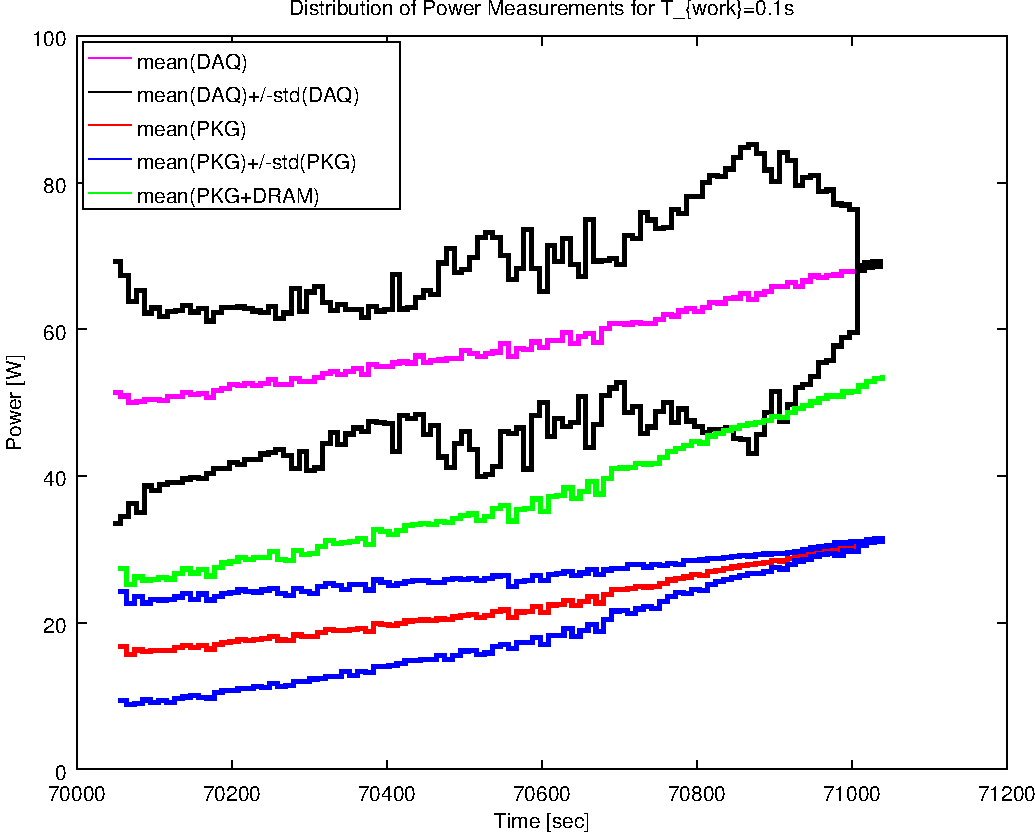
\includegraphics[width=\textwidth]{insertDelayTw100msCropped}
    \caption{Simulation Results}
    \label{simulationfigure}
\end{figure}

\section{Conclusion}
Write your conclusion here.

\end{document}
